% =========================================================
\chapter{Week1 : Part B}
% =========================================================

\section{Mobile Platforms}

\begin{defnbox}[title=Mobile platform]
The ingredients that come together to enable the \textbf{creation}, \textbf{distribution},
and \textbf{operation} of mobile content and services.
\end{defnbox}

\begin{center}
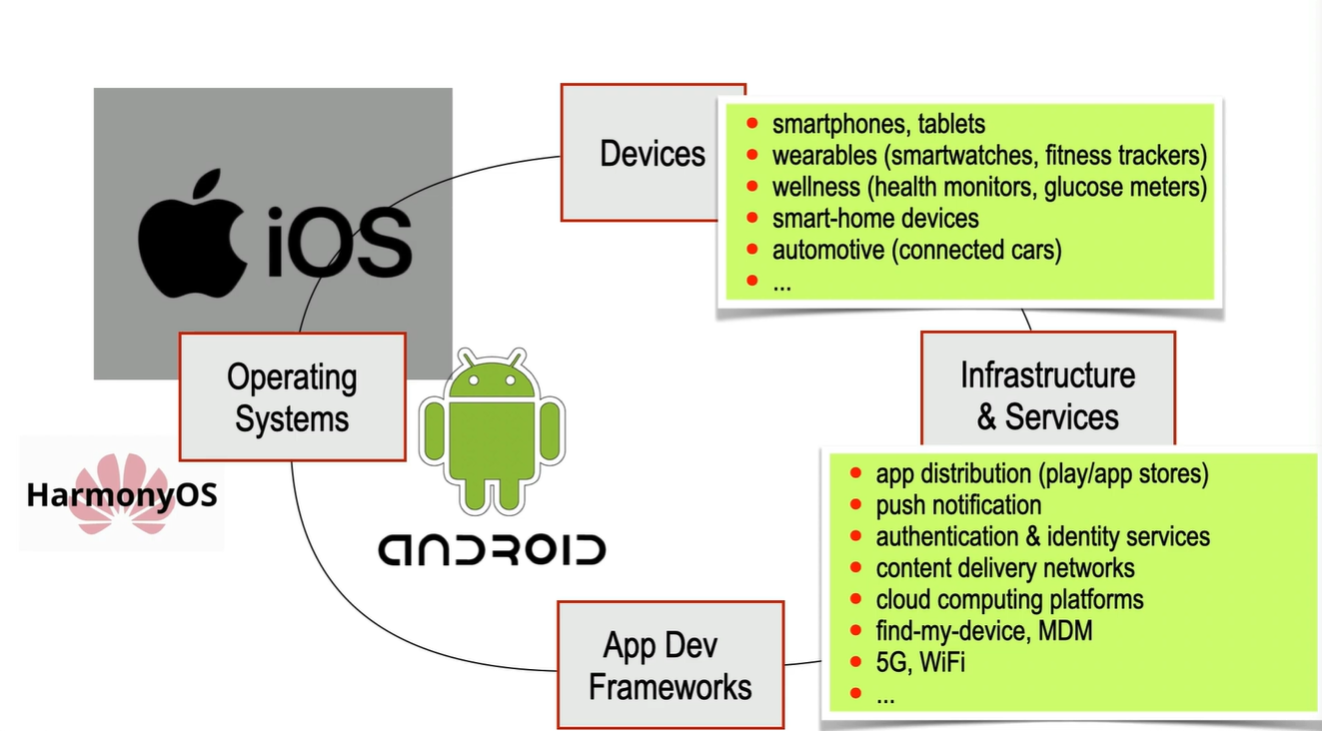
\includegraphics[width=\linewidth]{images/mobile-platform.png}
\end{center}

\section{The Mobile Device}

\subsection{The Mobile SoC = A "Commitee" of Processors}

\begin{defnbox}[title=Mobile SoC (System-on-Chip)]
A single chip integrating many specialized processors, each optimized for a different job. This heterogeneity is what lets a phone deliver serious compute for a few Watts.
\end{defnbox}

\begin{center}
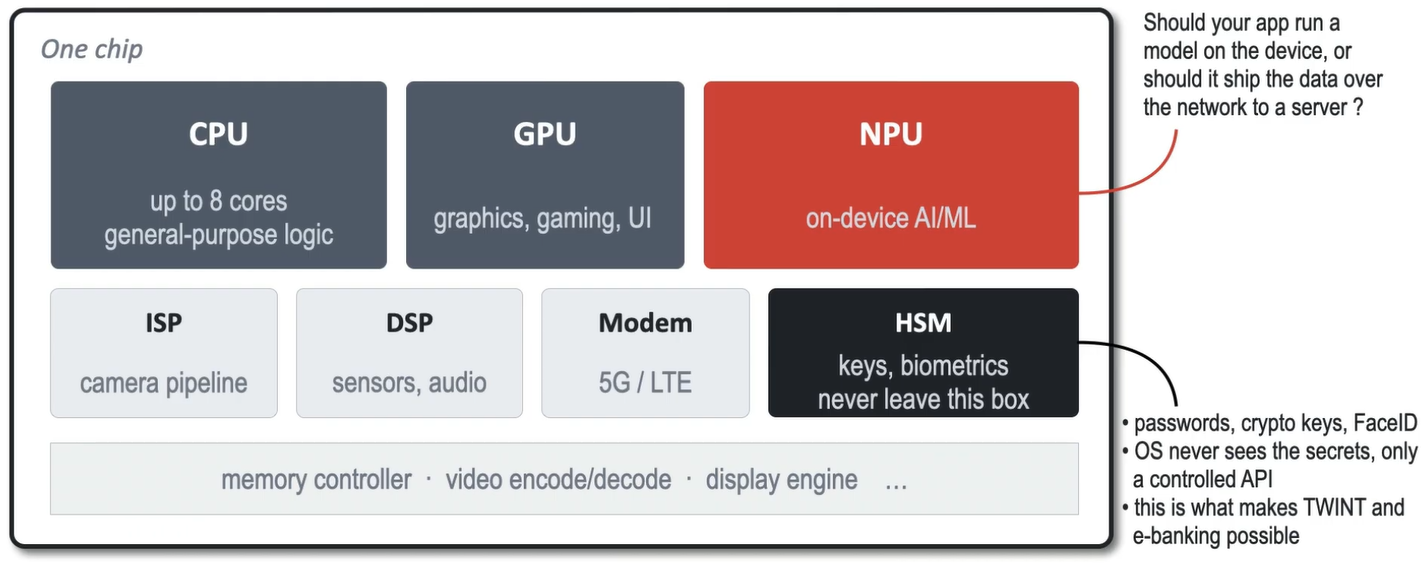
\includegraphics[width=\linewidth]{images/mobile-SoC.png}
\end{center}

\begin{keybox}[title=On-device vs. server]
The NPU raises a design question for every app that uses ML: should the model run on the device, or should the data be shipped over the network to a server?
\end{keybox}

\begin{keybox}[title=Why the HSM matters]
\begin{itemize}
  \item Stores passwords, crypto keys, FaceID data.
  \item The OS neever sees the secrets, only a controlled API.
  \item This isolation is what makes TWINT and e-banking possible.
\end{itemize}
\end{keybox}

\subsection{Fragmentation}

\begin{center}
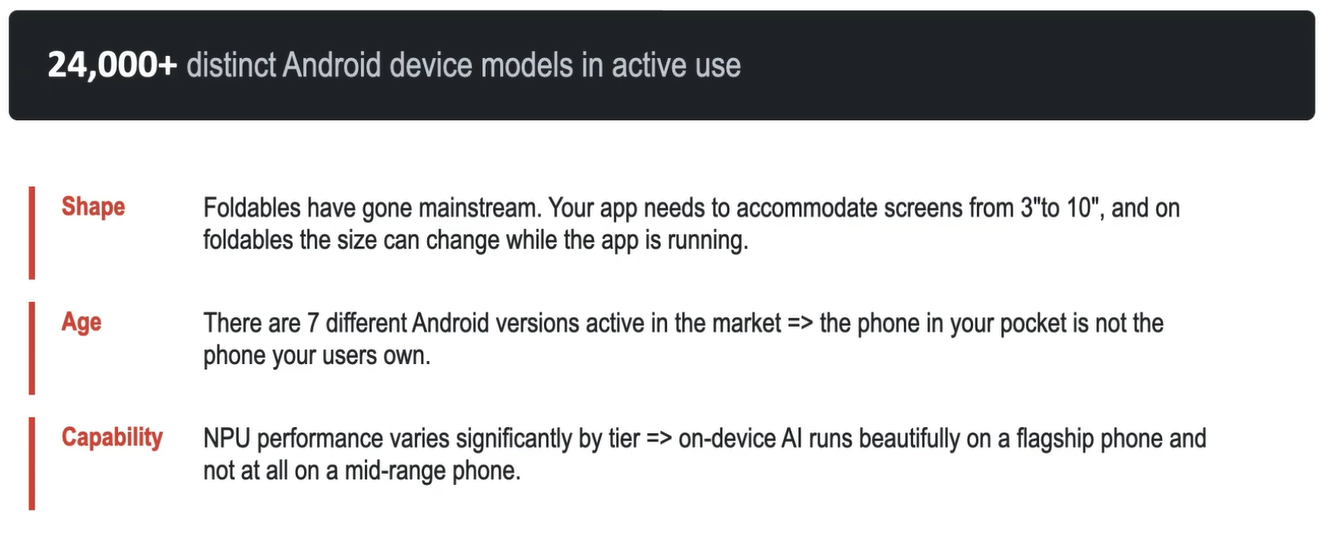
\includegraphics[width=\linewidth]{images/fragmentation.png}
\end{center}

\begin{warnbox}
How do you make your app work across the board?
\end{warnbox}

\section{Mobile OS vs Server OS}

\subsection{User Model and Security}

\begin{center}
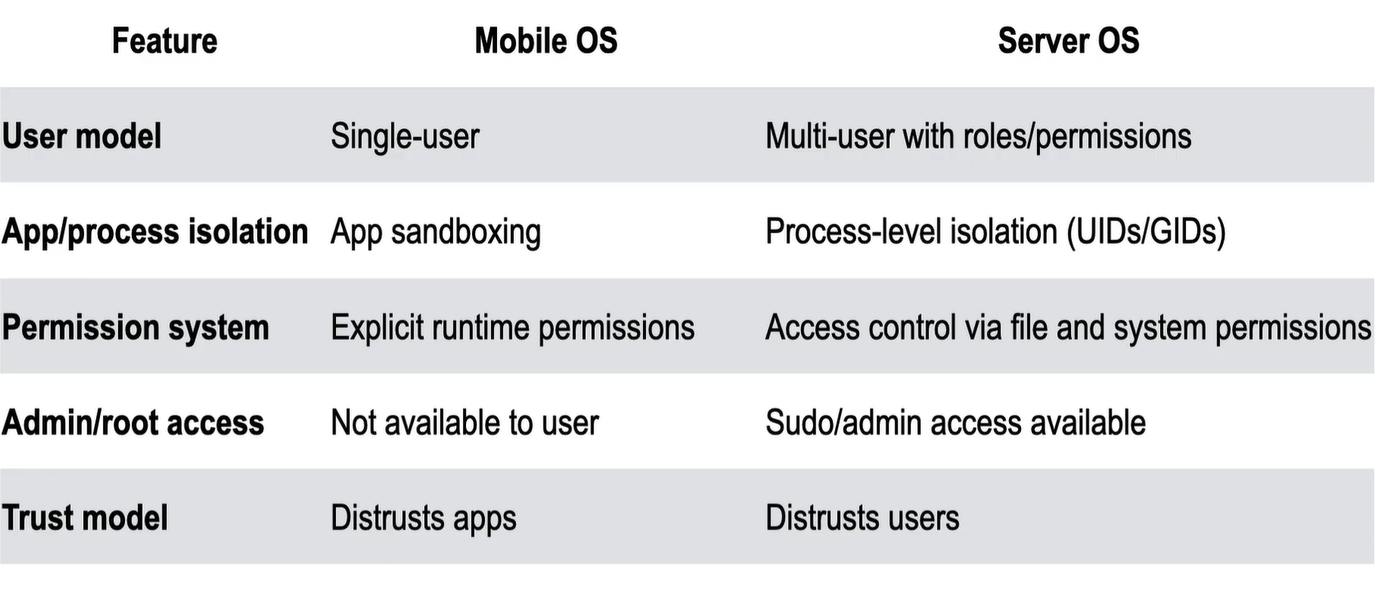
\includegraphics[width=\linewidth]{images/user-model-security.png}
\end{center}

\subsection{Power Management}

\begin{center}
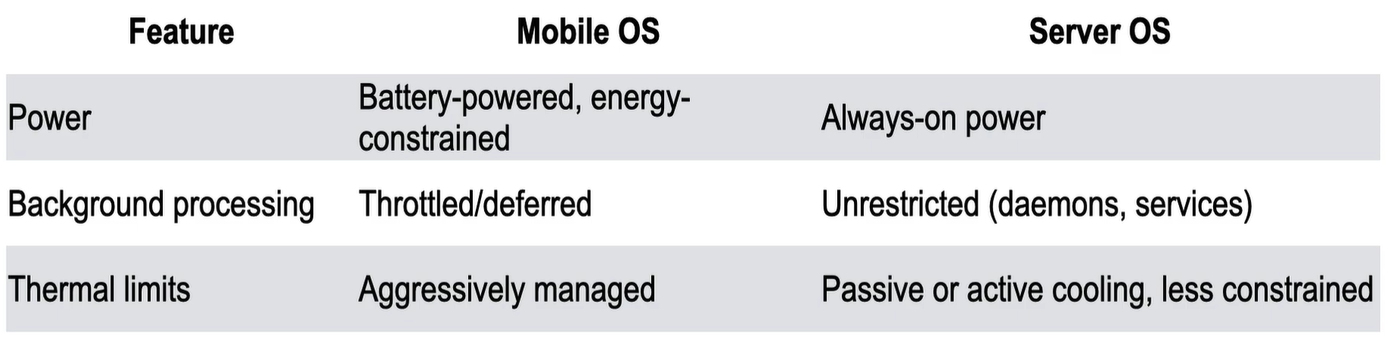
\includegraphics[width=\linewidth]{images/power-management.png}
\end{center}

\subsection{Execution Model \& App Lifecycle}

\begin{center}
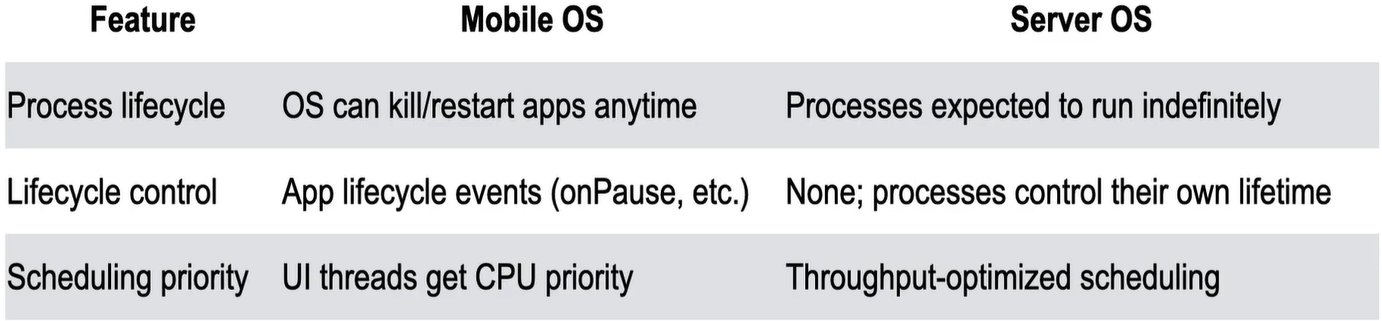
\includegraphics[width=\linewidth]{images/execution-model-n-app-lifecycle.png}
\end{center}

\subsection{Network \& Connectivity}

\begin{center}
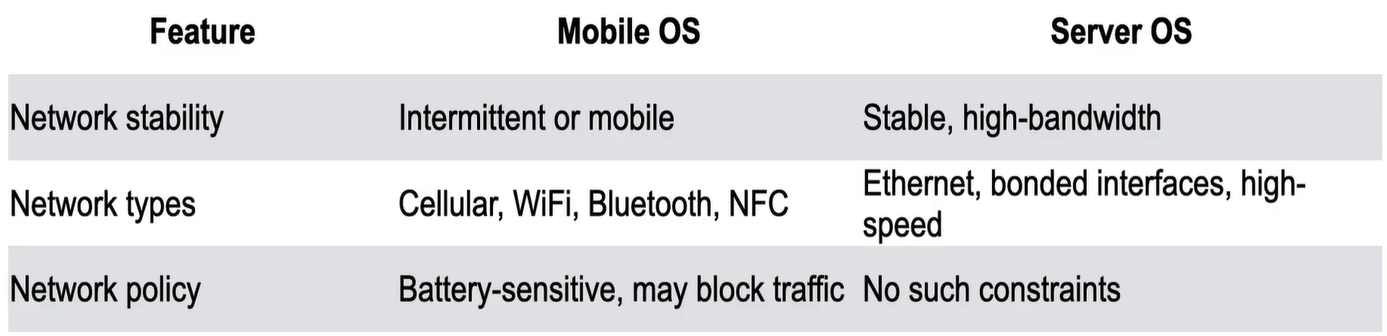
\includegraphics[width=\linewidth]{images/network-n-connectivity.png}
\end{center}

\subsection{UI \& Input/Ouput}

\begin{center}
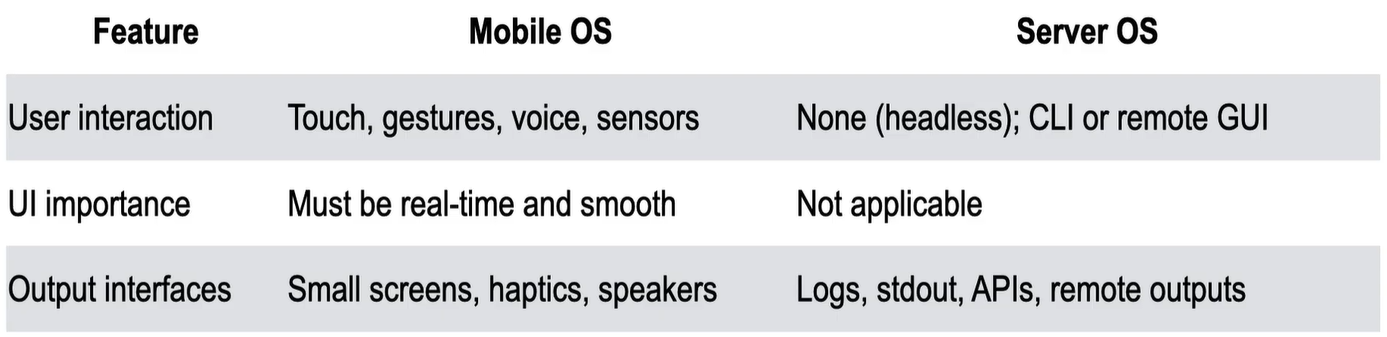
\includegraphics[width=\linewidth]{images/ui-n-io.png}
\end{center}

\subsection{Storage \& Filesystem}

\begin{center}
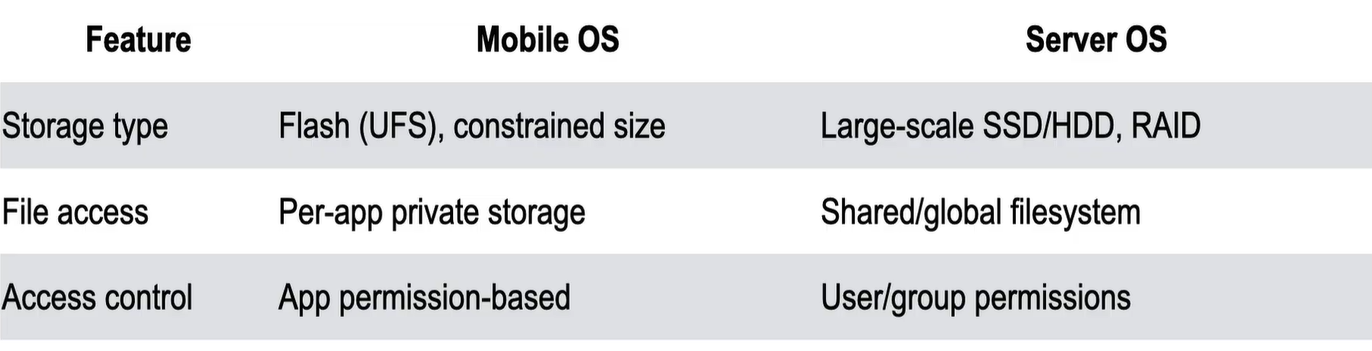
\includegraphics[width=\linewidth]{images/storage-n-fs.png}
\end{center}

\subsection{Hardware Environment}

\begin{center}
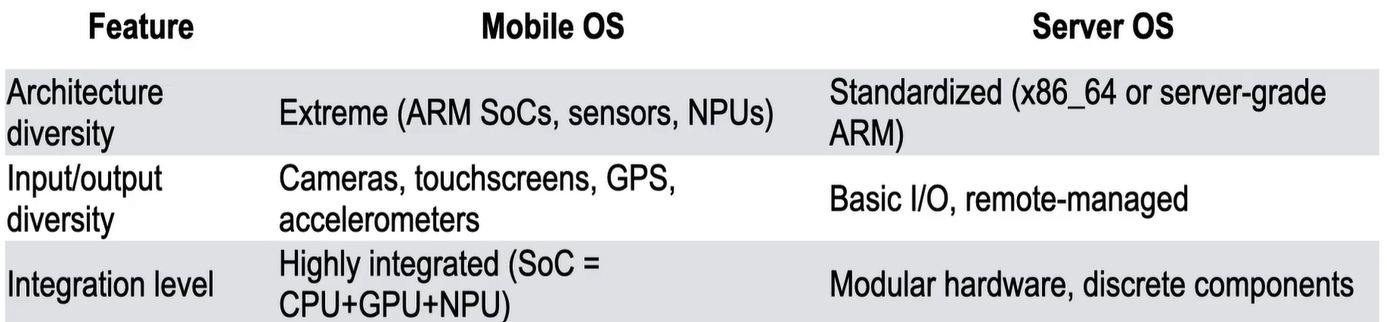
\includegraphics[width=\linewidth]{images/hardware-environment.png}
\end{center}

\subsection{Software Updates \& Maintenance}

\begin{center}
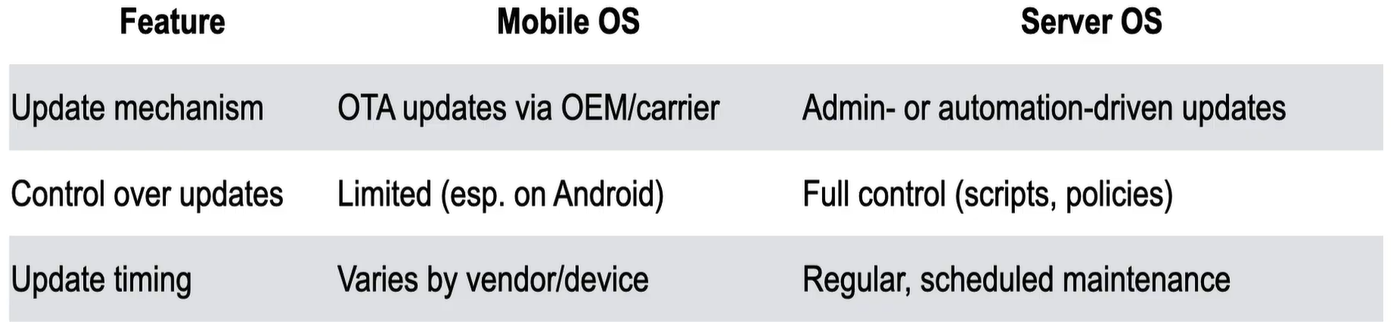
\includegraphics[width=\linewidth]{images/sofw-updates-n-maintenance.png}
\end{center}

\subsection{Difference between Android/IOS}

\begin{center}
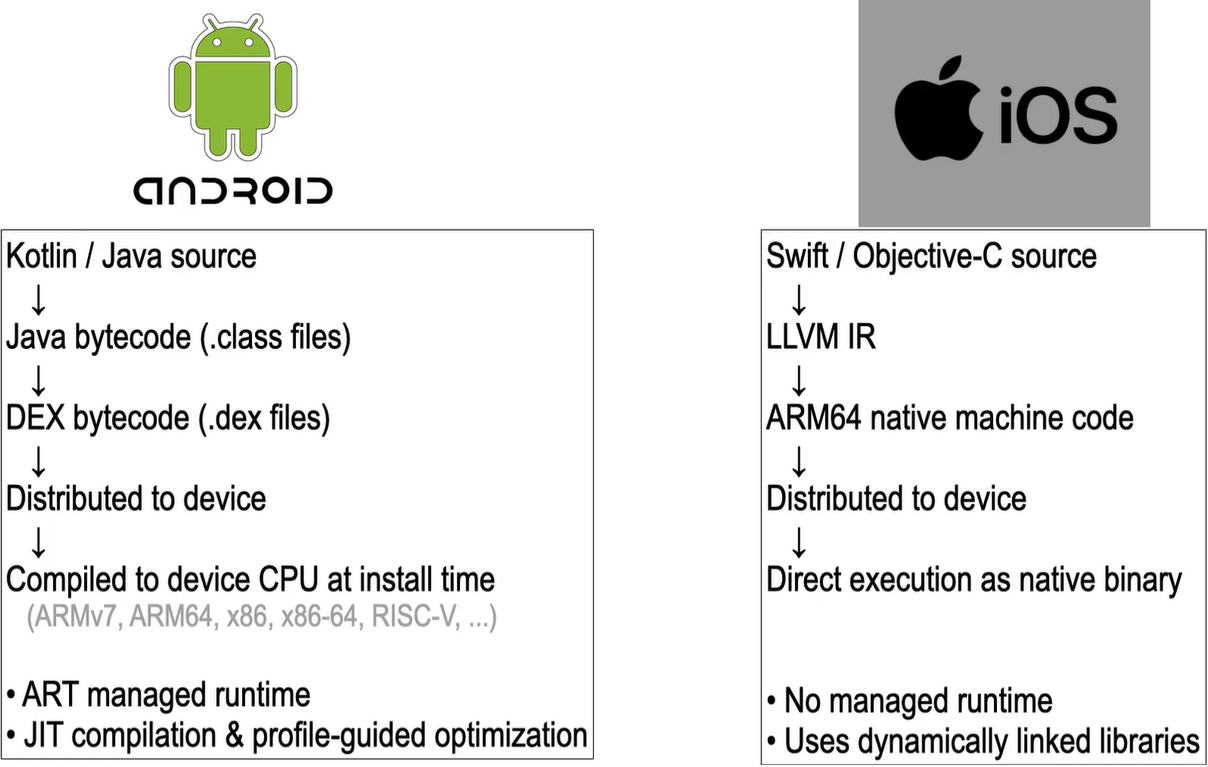
\includegraphics[width=\linewidth]{images/diff-android-ios.png}
\end{center}

\section{App Data (Persistence Levels)}

\begin{center}
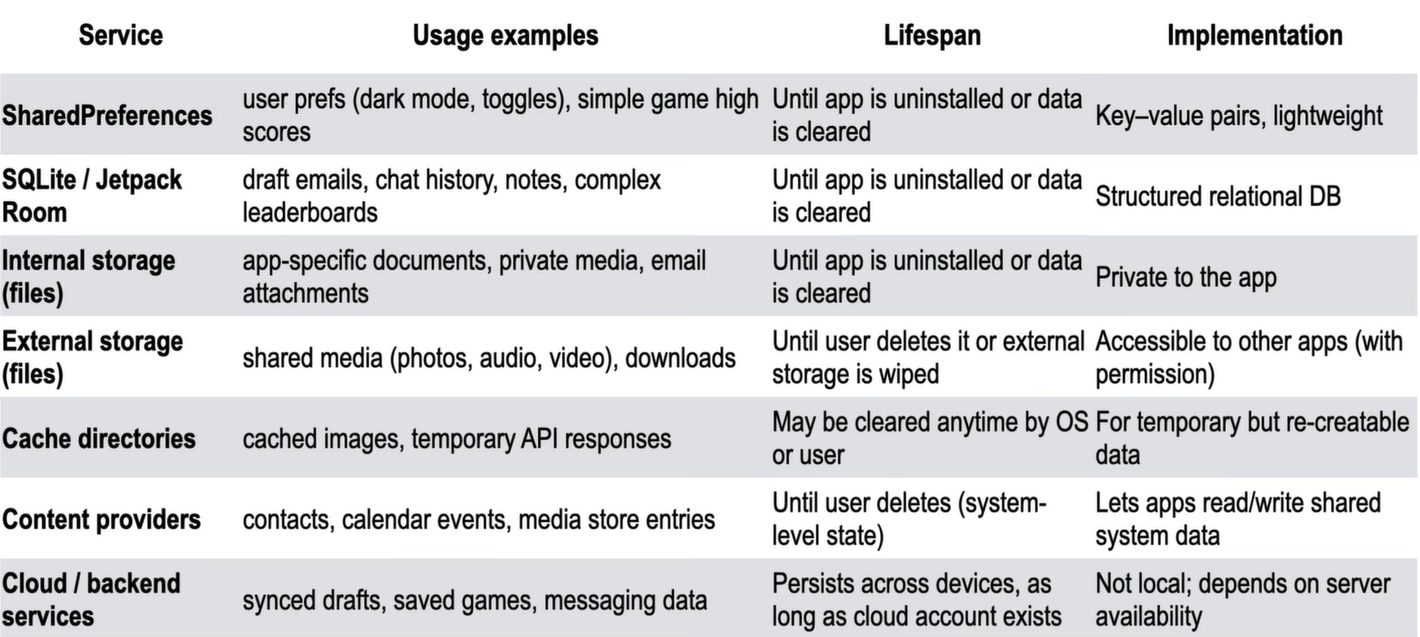
\includegraphics[width=\linewidth]{images/app-data.png}
\end{center}

\begin{exbox}[title=Which row survives what?]
Say your app remembers the user's favorite restaurants.
\begin{itemize}
  \item Which row should it use to survive a \textbf{reinstall of the app}?
  \item Which row should it use to survive a reinstall on a \textbf{new phone}?
\end{itemize}
\end{exbox}

\begin{keybox}[title=Answer]
\begin{itemize}
  \item \textbf{Survives reinstall (same phone):} SharedPreferences, Room and internal storage all die on uninstall. External storage and cloud storage both survive.
  \item \textbf{Survives reinstall on a new phone:} external storage won't work, since it never existed on that phone in the first place. Only \textbf{cloud storage} works.
\end{itemize}
Choose the storage service based on data complexity, visibility, and required lifespan -- a real project will typically combine more than one row of this table.
\end{keybox}

\section{The Split-App Model}

\begin{itemize}
  \item \textbf{Client-side (frontend)}
  \begin{itemize}
    \item runs on the user's device, provides the UI and UX
  \end{itemize}
  \item \textbf{Server-side (backend)}
  \begin{itemize}
    \item runs on a server or in the cloud
  \end{itemize}
  \item \textbf{Client interacts with cloud services}
  \begin{itemize}
    \item typically REST APIs or GraphQL
    \item send HTTP request
    \item get back JSON or XML
  \end{itemize}
\end{itemize}

\subsection{Benefits of Split-App Model}

\begin{propbox}
Modularity + contracts between the frontend and backend $\Rightarrow$ highly decoupled $\Rightarrow$
\begin{itemize}
  \item Independent development
  \item Scalability
  \item Flexibility to choose the most suitable technology and frameworks
  \item Can update app frontend independently of backend
  \item Reuse backend services across clients (mobile, Web, etc.)
\end{itemize}
\end{propbox}

\subsection{Backend/Network Services}

\begin{itemize}
  \item \textbf{Authentication and authorization}
  \begin{itemize}
    \item user sign-up, sign-in, and sign-out processes; access control and permissions
  \end{itemize}
  \item \textbf{Data storage and mgmt}
  \begin{itemize}
    \item user data and app content, typically with a CRUD interface
  \end{itemize}
  \item \textbf{Real-time data sync}
  \begin{itemize}
    \item real-time updates of data across user devices
  \end{itemize}
  \item \textbf{Payment processing}
  \begin{itemize}
    \item in-app purchases, subscriptions, payment verification and receipts
  \end{itemize}
  \item Content Delivery Networks (CDNs)
  \item Analytics and reporting
  \item Email and SMS
  \item Backup and recovery
  \item Geo-location
  \item Integration services
  \item \ldots
\end{itemize}

\subsection{Push Notifications}

\begin{itemize}
  \item Messages sent to the user by the backend of the app
  \item Each platform has its own push notification service
\end{itemize}

\begin{keybox}[title=Push notification flow]
\begin{itemize}
  \item \textbf{Push service registration:} the device requests a token from the platform's push service (Google/Apple), receives it, and registers that token with the app's backend (notification servers).
  \item \textbf{Routine delivery process:} the backend sends the notification to its push servers, which forward the message to the platform's push service, which delivers the push message to the device.
\end{itemize}
\end{keybox}

\section{MVVM}

\begin{center}
\begin{minipage}{0.45\linewidth}
\centering
\textbf{MVC (Model View Controller)}\\[2pt]
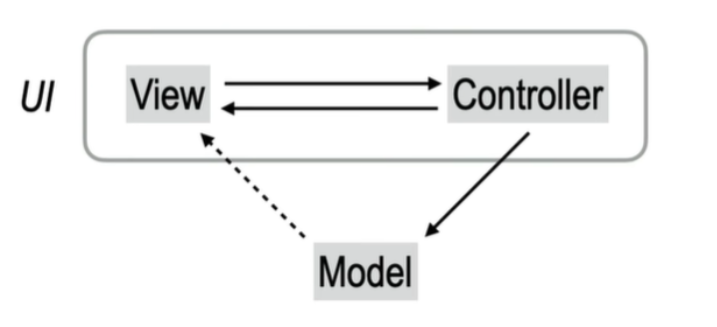
\includegraphics[width=\linewidth]{images/mvc.png}
\end{minipage}
\hfill
\begin{minipage}{0.45\linewidth}
\centering
\textbf{MVVM (Model View ViewModel)}\\[2pt]
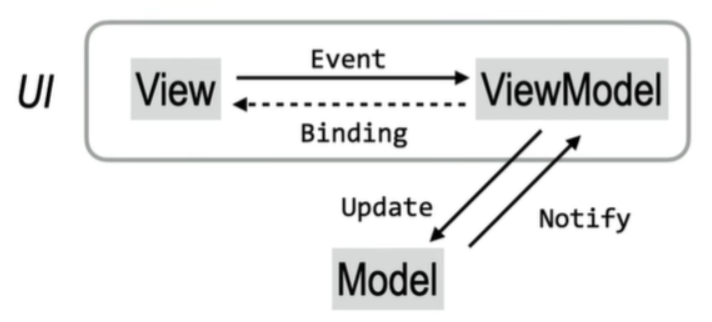
\includegraphics[width=\linewidth]{images/mvvm.png}
\end{minipage}
\end{center}

\begin{center}
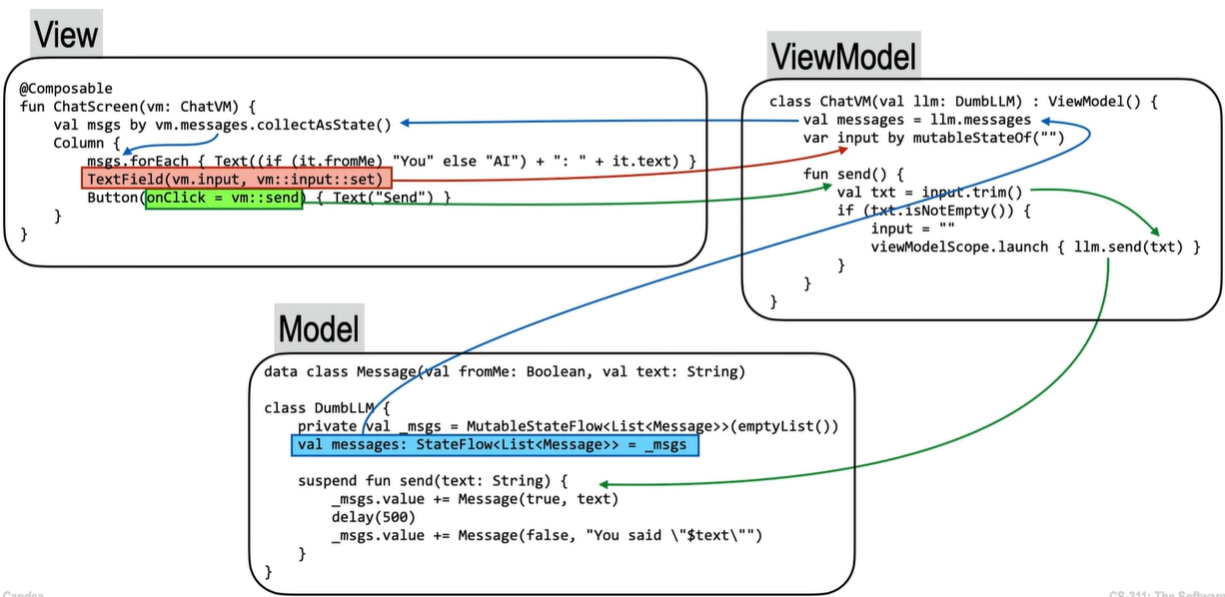
\includegraphics[width=\linewidth]{images/mvvm-example.png}
\end{center}

\begin{defnbox}[title=Observability]
Key concept in MVVM: enables communication between the app's data layer and its UI.
\begin{itemize}
  \item The view never pulls data directly from the view model; it reacts to changes pushed from the view model through the underlying mechanism.
  \item The view model exposes state; the UI functions in the view connect to this state; once bound, the framework recomposes the affected UI functions automatically whenever there's a state change.
  \item When the user interacts with the UI, the view calls the view model to communicate these user actions.
\end{itemize}
\end{defnbox}

\begin{rembox}
Layers are decoupled $\Rightarrow$ you can swap the model (e.g.\ dumb echo LLM for one calling OpenAI or a local model) or the view (e.g.\ phone UI for a web browser) without touching the other layers.
\end{rembox}

\begin{exbox}[title=Where does ``3 minutes ago'' belong?]
To show in the UI how long ago a message was sent (e.g.\ ``3 minutes ago''), which layer holds that functionality: the view, the view model, or the model?
\end{exbox}

\begin{keybox}[title=Answer: the view model]
\begin{itemize}
  \item The model keeps the timestamp of each message -- set once, it never changes.
  \item The string on screen changes every minute while the data sits still, so it can't be done in the model.
  \item Not in the view either: the moment the view does data arithmetic and runs a timer, you can't test any of it without launching a screen -- the view must stay stateless (re-creatable from the view model).
  \item The view model exists exactly for this kind of UI logic: to display ``3 minutes ago'' you need the model's timestamp plus a notion of the current time, both combined in the view model -- testable in milliseconds by feeding it various values of current time.
\end{itemize}
\textbf{Variant:} for a screen saying ``last refreshed 2 minutes ago'', the timestamp of the last refresh belongs in the view model instead of the model, because nobody sent that information and no other client cares -- purely UI state, nothing in the model.
\end{keybox}

\subsection{Benefits of MVVM}

\begin{itemize}
  \item Decouple UI logic from application's logic (``business logic'')
  \begin{itemize}
    \item View is conceptually a function of the ViewModel $\Rightarrow$ can be entirely computed from the ViewModel every time
    \item E.g., on mobile: app may run in background and need no UI --- can destroy View and re-create from the ViewModel whenever needed
  \end{itemize}
  \item Enables UIs that are reactive, responsive, dynamic
  \item Easy to test
  \item Easy to develop by separate people
  \item Easy to evolve, maintain, and reuse
\end{itemize}

\section{Components of A Mobile App}

\subsection{Four Android App Components}

\begin{itemize}
  \item \textbf{[1] Activities}
  \begin{itemize}
    \item Entry point for interacting with the user (1 screen + UI)
    \item One app can start an activity in another app (e.g., camera can email photo)
  \end{itemize}
  \item \textbf{[2] Services}
  \begin{itemize}
    \item Run in background without UI
    \item (often replaced or augmented by WorkManager for deferrable tasks)
  \end{itemize}
  \item \textbf{[3] Broadcast receivers}
  \begin{itemize}
    \item Receive ``out of band'' event broadcasts
    \item App doesn't need to be running to receive broadcast
  \end{itemize}
  \item \textbf{[4] Content providers}
  \begin{itemize}
    \item Manage data that is of interest to multiple apps
  \end{itemize}
\end{itemize}

\subsection{Activities}

\begin{itemize}
  \item Key part of an Android app
  \item Provides the window in which the app draws its UI
  \item UI consists of multiple screens
  \item Screens defined inside the main Activity
\end{itemize}

\subsection{Inter-App Communication via Intents}

\begin{itemize}
  \item An app can cause another app's component to start
  \begin{itemize}
    \item E.g., WhatsApp takes a photo with the Camera app
  \end{itemize}
  \item Activation is via an Intent object
  \begin{itemize}
    \item Think of it as an ``active message''
  \end{itemize}
  \item To start activities and services: \texttt{<action, URI>} $\rightarrow$ \underline{explicit} intent
  \begin{itemize}
    \item E.g., \texttt{<ACTION\_DIAL, "tel:123456789">}, \texttt{<ACTION\_WEB\_SEARCH, "app developers">}
  \end{itemize}
  \item Register for broadcast announcements: \texttt{<announcement>} $\rightarrow$ \underline{implicit} intent
  \begin{itemize}
    \item E.g., \texttt{<ACTION\_BATTERY\_LOW>}, \texttt{<ACTION\_POWER\_DISCONNECTED>}
  \end{itemize}
  \item For content providers: pull instead of push
  \begin{itemize}
    \item Activated by request from a \texttt{ContentResolver}
  \end{itemize}
\end{itemize}

\begin{center}
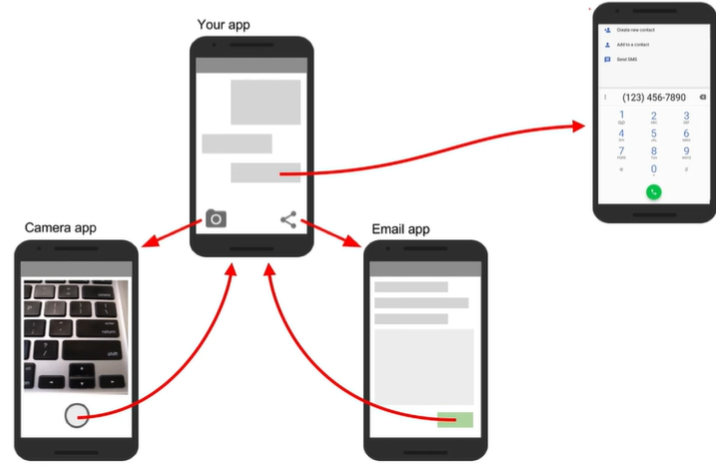
\includegraphics[width=0.7\linewidth]{images/inter-app.png}
\end{center}

\section{The Lifecycle of an Android Activity}

\begin{defnbox}[title=Single entry vs.\ multiple entry points]
A traditional program has one entry point, \texttt{main()}: in $\to$ runs $\to$ returns. An Android Activity instead exposes \textbf{seven} lifecycle callbacks, each a possible entry point -- and no single way out.
\end{defnbox}

\begin{center}
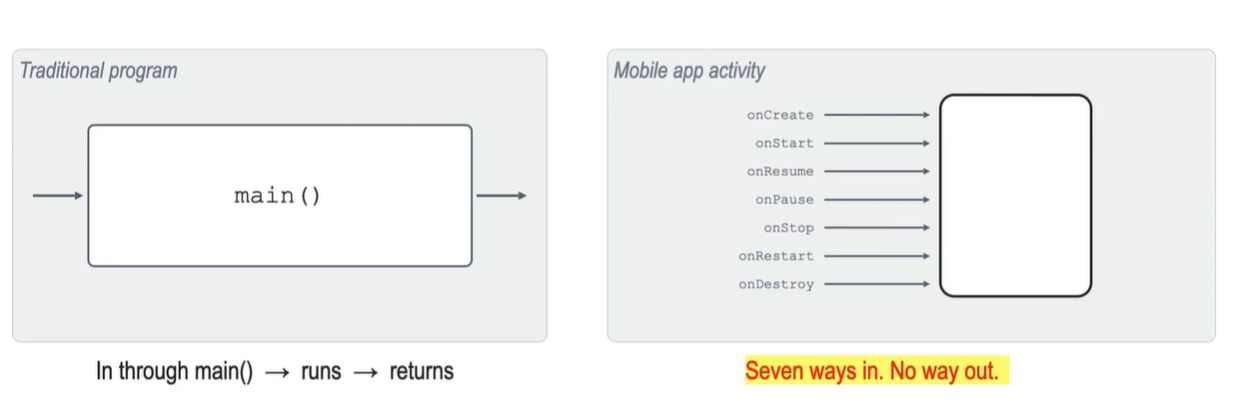
\includegraphics[width=\linewidth]{images/single-vs-multiple-entrypoints.png}
\end{center}

\begin{center}
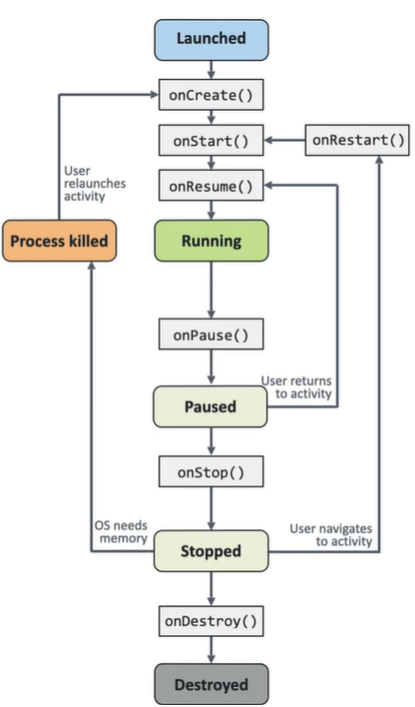
\includegraphics[width=0.55\linewidth]{images/lifecycle-activity.png}
\end{center}

\begin{exbox}[title=Rotating mid-form]
The user is halfway through filling in a form -- three fields done, typing the fourth -- then rotates the phone to landscape. Which callbacks fire from the start of the rotation until the form is back on screen, and what happens to the text typed so far?
\end{exbox}

\begin{keybox}[title=Answer]
The Activity object is destroyed completely, then a brand new one is created in landscape mode:
\[
\text{pause} \to \text{stop} \to \text{destroy} \to \text{create} \to \text{start} \to \text{resume}
\]
with a \textbf{different Activity object} and a different screen configuration -- anything kept in the Activity's own fields is gone.
\end{keybox}

\begin{rembox}[title=Why the form text survives anyway]
\begin{itemize}
  \item The \textbf{ViewModel} is deliberately scoped to outlive the Activity across a configuration change. If the form text lives in the ViewModel (as it should), the new Activity reads that state straight back -- separation of concerns at work.
  \item Redrawing itself is not a callback: a frame loop repaints the screen at 60--120\,Hz whenever something changed. The lifecycle governs whether the UI is drawable; the frame loop governs when pixels actually change.
\end{itemize}
\end{rembox}

\begin{warnbox}[title=A different risk: switching away]
Switching away from the app mid-form (not a rotation -- e.g.\ to take a call) risks the process itself being killed before it resumes. That kills everything, including the ViewModel. The only way to recover the text would be to persist it in \texttt{onStop} -- but a half-filled form generally isn't expected to survive this case.
\end{warnbox}

\begin{rembox}[title=iOS has a similar lifecycle]
Direct correspondences exist between the Android and iOS callbacks. Difference: iOS may enter a \textbf{suspended} state after being paused (stays in memory, executes no code); Android may keep the process alive with no explicit suspended state.
\end{rembox}

\begin{keybox}
Mobile app lifecycles are considerably more sophisticated than server or desktop ones -- a reflection of the added complexity and constraints mobile apps face.
\end{keybox}
